\partopening{Rebalancing and Traded Funds}{part:funds}
{How finite trading, costs, and liquidation change the expectation shortfall.}

\section{Finite rebalancing changes the classification}\label{sec:finitefunds}
The continuous-exposure result is not automatically a theorem about an
exchange-traded fund that resets its exposure once a day. Between reset
dates, the elementary contract holds fixed shares and a cash position.
This distinction changes the martingale classification even before fees,
financing, or tracking error are introduced.

Let $X$ be a continuous nonnegative $Q$-local martingale with $X_0=1$.
Over one holding interval, normalized gross wealth at exposure $\pi$ is
\begin{equation}\label{eq:oneholding}
 G_t^\pi=1-\pi+\pi X_t.
\end{equation}
Writing $\delta_T=1-\E_Q[X_T]$, linearity gives
\begin{equation}\label{eq:signedgap}
 1-\E_Q[G_T^\pi]=\pi\delta_T.
\end{equation}
For $\pi<0$ this is a negative signed gap when the underlying is strict.
It is not a negative bubble in a nonnegative asset: the affine contract
can itself become negative. Limited liability needs an additional rule.

\subsection{Finite grids with exposure between zero and one}
For a finite deterministic grid $0=t_0<\cdots<t_N=T$, define
\begin{equation}\label{eq:gridwealth}
 W_t=W_{t_i}\left(1-\pi+\pi\frac{X_t}{X_{t_i}}\right),
 \qquad t_i\leq t\leq t_{i+1},\quad X_{t_i}>0.
\end{equation}
When $X_{t_i}=0$, keep the remaining wealth in cash. For $0<\pi\leq1$,
the factors and the wealth remain nonnegative.

\begin{proposition}[Finite-grid inheritance]\label{prop:grid}
For $0<\pi\leq1$ and every finite grid, $W$ is a nonnegative continuous
local martingale and is a true martingale on $[0,T]$ exactly when $X$ is.
If $X$ is strict on that horizon, so is $W$.
\end{proposition}

The mechanism is the accumulated conditional expectation loss of each
holding. Define
$A_i=X_{t_i}-\E_Q[X_{t_{i+1}}\mid\mathcal F_{t_i}]\geq0$ and
$h_i=\pi W_{t_i}/X_{t_i}$ where the denominator is positive, zero
otherwise. Then
\begin{equation}\label{eq:lossdecomp}
 1-\E_Q[W_T]=\sum_{i=0}^{N-1}\E_Q[h_i A_i].
\end{equation}
Each summand is nonnegative. If $X$ is a martingale, every $A_i$ vanishes.
Conversely, induction gives a lower bound on the holding where $A_i$ can
be nonzero, and
$1-\E_Q[W_T]\geq\pi^N\delta_T$. This proves inheritance. The bound
can be extremely small and is generally useful for classification rather
than for monetary estimation.

The two examples in Part~\ref{part:theory} now become a comparison of
trading rules.
\begin{table}[htbp]\centering\small
\begin{tabularx}{\linewidth}{@{}YYYY@{}}\toprule
Underlying, $\pi=1/4$ & Asset & Every finite grid & Continuous wealth\\
\midrule
Absorbed Brownian, $\sigma=1$ & Martingale & Martingale & Strict\\
Reciprocal-Bessel type, $\sigma=x^2$ & Strict & Strict & Martingale\\
\bottomrule\end{tabularx}
\caption{The discrete/continuous reversal under the stated wealth and
post-default conventions. These are pricing-measure classifications.}
\label{tab:reversal}
\end{table}

At default, a finite-grid fund preserves the cash fraction left from the
last rebalance. The continuous model keeps replenishing the risky
fraction as the price approaches zero. In the absorbed Brownian example,
every finite-grid terminal mean is one while the continuous mean is
smaller, so the terminal values cannot converge in $L^1$. This does not
by itself rule out weaker modes of convergence through absorption.
\source{claims 004, 005, and 001. The stochastic inputs are finite trading,
bounded stopping, and the nonnegative-local-martingale supermartingale property}

\subsection{Refinement and the size of the discrepancy}
Away from zero, standard stability of stochastic differential equations
gives convergence of the grid recursion to the stochastic exponential as
the mesh shrinks \cite{emery1979lipschitz}. Localizing to
$X\in(1/m,m)$ gives uniform convergence in probability on a finite
horizon. If $X$ stays strictly positive throughout the horizon, the stop
can be removed. The stability theorem supplies the path-convergence step.

Path convergence does not alone ensure convergence of expectations of
unbounded payoffs. Bounded Lipschitz functionals, including puts on
nonnegative wealth, have converging expectations. Calls require additional
tail control. For $0\leq\pi\leq1$ and
$Q(X_t>0\text{ for all }t\in[0,T])=1$, a mean-one continuous limit
supplies that control automatically:
\begin{equation}\label{eq:meanone}
 \E_Q[V_T^\pi]=1\quad\Longrightarrow\quad
 \E_Q|W_T^{(n)}-V_T^\pi|\longrightarrow0.
\end{equation}
Fatou's lemma and the bound $\E_Q[W_T^{(n)}]\leq1$ force the means to
converge to one; the nonnegative shortfall then gives $L^1$ convergence.
All Lipschitz payoff expectation prices, calls included, converge.

For $\sigma=x^2$ and $\pi=1/4$, every finite-grid fund is strict yet its
defect tends to zero. Binary classification can therefore differ at every
finite frequency while the valuation discrepancy disappears. When the
continuous limit is strict, the existing result gives only a one-sided
bound on the limiting defect, not full convergence. A numerical study at
$\pi=3/4$ finds means approximately $0.786$, $0.819$, and $0.833$ for
4, 64, and 1,008 intervals, approaching the continuous value $0.8465$.
That pattern is evidence in one model; it cannot exclude probability mass
in paths too rare for the numerical calculation to resolve.
\source{claims 007 and 009; experiment 012}

\section{Leverage, inverse exposure, and liquidation}\label{sec:liquidation}
For $\pi>1$, a sufficiently large decline makes
\eqref{eq:oneholding} negative. For $\pi<0$, a sufficiently large rise does
the same. A model of a nonnegative fund must say what happens at that
point. Resetting the exposure at the next date is not enough to specify
limited liability between dates.

\subsection{Inverse funds under an explicit floor rule}
Let $W$ now be the signed finite-grid recursion at $\pi<0$. Fix
$0\leq a<1$ and liquidate into cash at the first continuous crossing
below the floor $a$, capped at $T$. By continuity, wealth at an actual
crossing is $a$. Denote stopped wealth by $H^a$. On a grid with $N$
intervals,
\begin{equation}\label{eq:inversebound}
 a\leq H_t^a\leq(1-\pi)^N.
\end{equation}
A bounded local martingale is a uniformly integrable martingale.
Thus this finite-grid, continuously liquidated inverse fund has no
defect, even when its underlying is strict.

For example, at $\pi=-1$ on one interval, liquidating when $X$ first
exceeds $3/2$ preserves wealth between $1/2$ and $2$. The underlying
$\mathrm{d}X=X^2\mathrm{d}W$ can be strict while the liquidated inverse
contract is a martingale. This is an implication of the contract rule,
not evidence that inverse exposure removes every economically relevant
risk.

\subsection{Leveraged-long funds}
For $\pi>1$, impose the same floor rule and write
$d_H=1-\E_Q[H_T^a]$. The lab establishes
\begin{equation}\label{eq:longbound}
 a\leq H_t^a\leq a+\pi^N X_t,
 \qquad 0\leq d_H\leq1-a,
 \qquad d_H\leq\pi^N\delta_T.
\end{equation}
Hence a true-martingale underlying gives a true-martingale liquidated
fund. A positive fund defect implies a positive underlying defect, but
the converse is not established. Since $\pi^N$ grows rapidly, the
quantitative lower bound $\delta_T\geq d_H/\pi^N$ is weak at daily
rebalancing frequencies.

In the registered simulations, leveraged-long funds over two strict
underlyings retain defects of roughly 0.40--0.96 at daily rebalancing
for exposures 1.5--3 with a zero floor, and 0.36--0.50 with a half-wealth
floor. Inverse funds over the strict underlyings are consistent with zero.
High-leverage geometric-Brownian controls are less stable: some inverse
cells are unresolved and the long controls at exposure three are fragile
individually. The large long-fund effects are results for these chosen
models and floor rules.
\source{claims 011 and 018; experiments 017--018}

\subsection{Costs are not a bubble}
If terminal net wealth is $Y_T=W_T-c_T+e_T$, where costs have expected
value $d_T$ under $Q$ and $\E_Q|e_T|\leq\varepsilon$, then
\begin{equation}\label{eq:cost}
 \left|(1-\E_Q[Y_T])-(1-\E_Q[W_T])-d_T\right|\leq\varepsilon.
\end{equation}
Expense, borrowing, and financing terms can be incorporated into the
one-interval return accounting, following the leveraged-fund framework
of Avellaneda and Zhang \cite{avellaneda2009path}. A deterministic fee
can lower expected net wealth without any strict-local-martingale
mechanism. An expected tracking bound under $P$ does not automatically
provide the required bound under $Q$.

The measured ETF data put a scale on these adjustments. Across eight
leveraged and inverse funds on QQQ and SPY, leveraged-long funds lose an
additional 0.6--1.7\% per year beyond the expense ratio, and inverse funds
0.1--1.1\%, measured against the total-return underlying. Reported standard
errors are 0.1--0.4 percentage points per year. Using a price index instead
would misread distributions as a cost. This is useful return accounting:
it separates ordinary financing and tracking effects from the expectation
shortfall studied in the theoretical model.
\source{claim 004; experiment 007}

\section{What discrete monitoring misses}\label{sec:monitorfloor}
Liquidation is path dependent. A simulated path can cross a boundary and
recover between observations. A program that looks only at observation
times can keep a fund alive after the continuously monitored contract
has terminated.

\begin{figure}[htbp]\centering
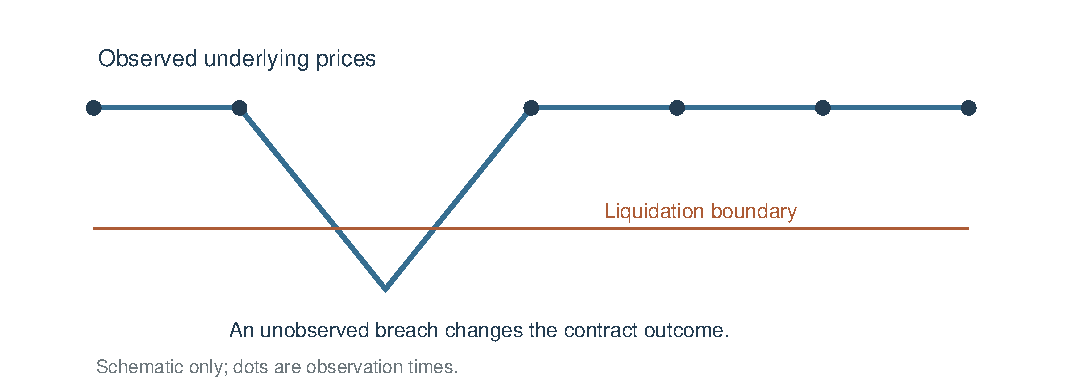
\includegraphics[width=\linewidth]{generated/missed_liquidation.pdf}
\caption{A boundary breach can be invisible at every observation time.
This is an explanatory schematic, not a simulated or historical record.}
\label{fig:floor}
\end{figure}

For monitoring times $F$ containing all rebalancing dates and $T$, define
a numerical quantity $Z_F$: if a sampled value of the signed recursion
is below $a$, replace terminal wealth by $a$; otherwise keep $W_T$.
This clipping is an artificial cash adjustment, not an executable trading
strategy. It has the useful pathwise property
\begin{equation}\label{eq:clip}
 a\leq H_T^a\leq Z_F,\qquad
 1-\E_Q[Z_F]\leq d_H.
\end{equation}
Adding monitoring times can only decrease $Z_F$. On a fixed rebalancing
grid, dense monitoring gives $L^1$ convergence to continuously
liquidated wealth under the stated models.

There is no uniform error rate based on the mesh alone over all
continuous paths. For any finite set of monitoring times, insert an
unobserved downward excursion in a gap. With one interval, $\pi=2$,
and $a=1/2$, a path observed at $X=1$ but dipping to $X=1/2$ in between
has $Z_F=1$ and liquidated terminal wealth $H_T^a=1/2$. Continuity
alone places no bound on how narrow the excursion can be.

This result gives a constructive numerical lesson. The particular clipped
quantity bounds the defect from below in expectation; freezing wealth at
the first sampled overshoot generally does not. A positive Monte Carlo
estimate still has sampling and discretization error, so it is evidence
for a positive lower bound, not a proof of its sign. The fund simulations
use this distinction to check the direction of monitoring bias.
\source{claim 020; experiment 018}
